%-------------------------------------------------------------------------------
% File: synth_results.tex
%
% Author: Marco Pinna
%         Created on 16/04/2022
%-------------------------------------------------------------------------------
\chapter{Synthesis results}\label{ch:synth_results}
This chapter concerns the automated logic synthesis process on the Xilinx Vivado Design Suite. The synthesis was performed using a Xilinx Zynq-7000 general purpose board (xc7z010clg400-1) as a target SoC.\\
Due to an insufficient number of I/O pins available on the actual board with respect to the ones requested by the specifications, the \textbf{implementation phase} was not carried out. Nevertheless, some results regarding resource usage, maximum clock frequency, critical path and power consumption could still be obtained during the synthesis phase.

\section{Bitwise architecture synthesis}
The synthesis process on Vivado showed no errors or warnings.\\

\subsection{Timing report}
After adding a time constraint for a clock period of 8 ns (125 MHz), the synthesis was re-run to obtain the timing report, whose summary is shown below:

\begin{figure}[H]
    \begin{center}
        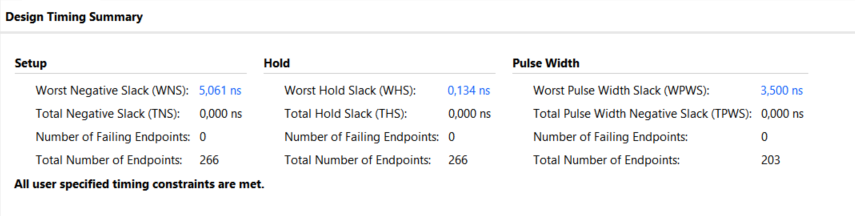
\includegraphics[scale=.75,clip]{img/vivado_bit_timing.png}
    \end{center}
    \vspace*{-0.5cm}
    \caption{Vivado timing report summary for the bitwise architecture synthesis}
    \label{fig:vivado_bit_timing}
\end{figure}

The Worst Negative Slack (WNS)is determined by the critical path of the circuit, which is highlighted in the figure below:

\begin{figure}[H]
    \begin{center}
        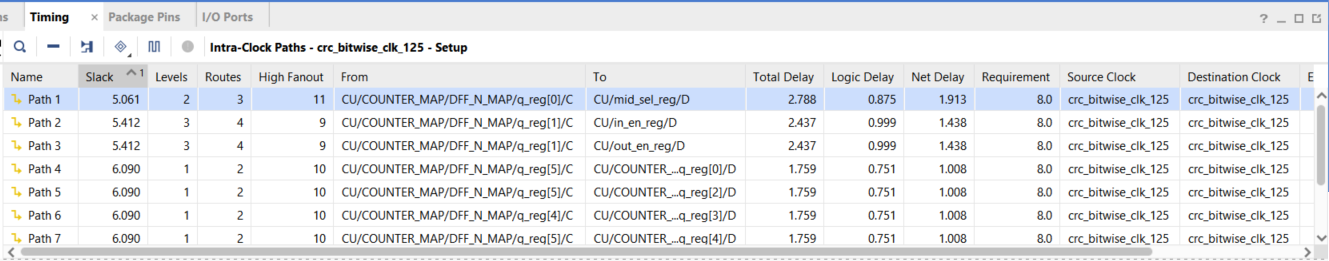
\includegraphics[scale=.5,clip]{img/vivado_bit_critical_path.png}
    \end{center}
    \vspace*{-0.5cm}
    \caption{Critical path of the bitwise architecture synthesis}
    \label{fig:vivado_bit_critical_path}
\end{figure}
\hfill \break
The figure shows that the critical path of the architecture is inside the Control Unit component.\\
Since the WNS has a positive value, this means that the board can be driven at a higher frequency than the one set in the timing constraints file.\\
The maximum allowed frequency can be computed with the following formula

\begin{equation}\label{eq:max_freq}
f_{max} = \frac{1}{T_{clk} - WSN} = \frac{1}{8 ns - 5,061 ns} = \frac{1}{2,939 ns} \approx 340,25 MHz
\end{equation}
\hfill \break
which is compatible with the 667 MHz maximum frequency stated in the board datasheet.\\
A simple computation can provide the throughput of the bitwise algorithm implementation: since every computation requires 58 clock cycles, the maximum number of CRCs that can be computed in a second is

\begin{equation}\label{eq:CRC_per_second}
R_{CRC} = \frac{f_{max}}{58} \approx 5866379
\end{equation}
\hfill \break
which, in terms of bit throughput, corresponds to approximately 328.52 Mbit/s.

\subsection{Resource utilization report}

The following figure shows a summary of the resource utilization report for the bitwise architecture.

\begin{figure}[H]
    \begin{center}
        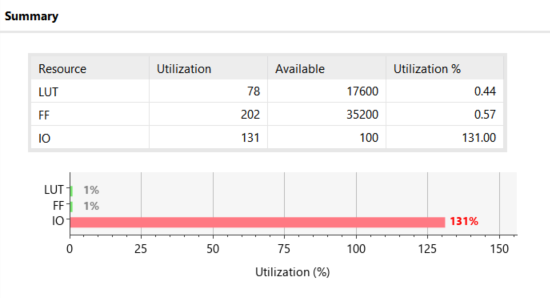
\includegraphics[scale=.75,clip]{img/vivado_bit_resources.png}
    \end{center}
    \vspace*{-0.5cm}
    \caption{Summary of the resource utilization report of the bitwise architecture}
    \label{fig:vivado_bit_resources}
\end{figure}
\hfill \break
As mentioned at the beginning of the chapter, the IO utilization exceeds 100\% since the specifications require a total of 131 ports while the IOB on the board amount to 100.\\
The LUT and FF utilization, on the other hand, is very low, standing at around 0.5\%.

\subsection{Power consumption report}

The following figure shows a summary of the power consumption utilization report for the bitwise architecture.

\begin{figure}[H]
    \begin{center}
        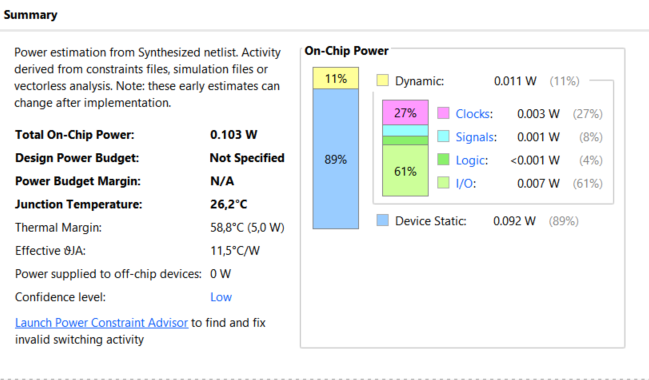
\includegraphics[scale=.85,clip]{img/vivado_bit_power.png}
    \end{center}
    \vspace*{-0.5cm}
    \caption{Summary of the power consumption report of the bitwise architecture}
    \label{fig:vivado_bit_power}
\end{figure}
\hfill \break
As it can be seen in the figure, the total power absorbed by the chip is around 0.1 W, most of which is static power consumption. This data however has to be taken with a grain of salt, since, as also stated in the figure, it has a low confidence level and the estimates could change after implementation.

\section{LUT-based architecture synthesis}
The same exact procedure was followed for the LUT-based architecture.\\
\hfill \break
The synthesis process on Vivado showed no errors or warnings.\\

\subsection{Timing report}
After adding a time constraint for a clock period of 8 ns (125 MHz), the synthesis was re-run to obtain the timing report, whose summary is shown below:

\begin{figure}[H]
    \begin{center}
        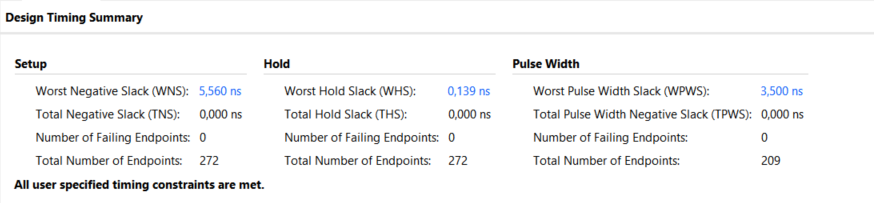
\includegraphics[scale=.75,clip]{img/vivado_lut_timing.png}
    \end{center}
    \vspace*{-0.5cm}
    \caption{Vivado timing report summary for the LUT-based architecture synthesis}
    \label{fig:vivado_bit_timing}
\end{figure}
\hfill \break
The Worst Negative Slack (WNS) has increased with respect to the bitwise architecture. The critical path of the circuit is highlighted in the figure below:

\begin{figure}[H]
    \begin{center}
        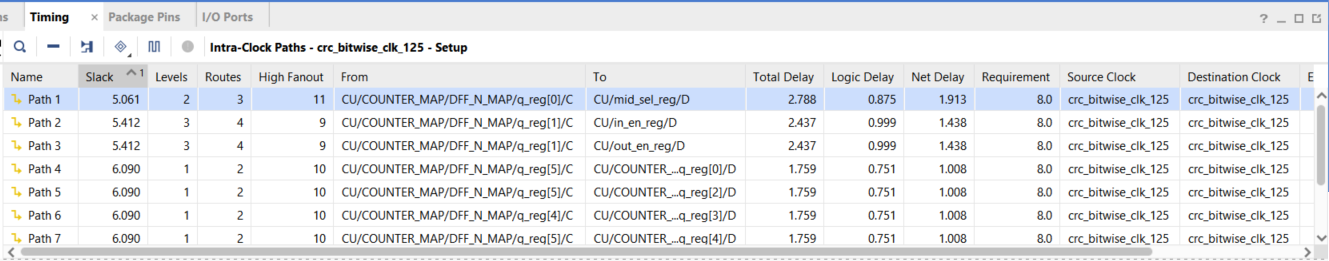
\includegraphics[scale=.5,clip]{img/vivado_bit_critical_path.png}
    \end{center}
    \vspace*{-0.5cm}
    \caption{Critical path of the bitwise architecture synthesis}
    \label{fig:vivado_bit_critical_path}
\end{figure}
\hfill \break
The figure shows that the critical path is now inside the PIPOShiftRegister.\\
Since in this case too the WNS has a positive value, this means that the board can be driven at a higher frequency than the one set in the timing constraints file.\\
Again, we can compute the maximum allowed frequency:

\begin{equation}\label{eq:max_freq}
f_{max} = \frac{1}{T_{clk} - WSN} = \frac{1}{8 ns - 5,560 ns} = \frac{1}{2,44 ns} \approx 409,84 MHz
\end{equation}
\hfill \break
which is higher than the other one and still compatible with the 667 MHz maximum frequency stated in the board datasheet.\\
\hfill \break
The throughput of the LUT-based algorithm implementation in terms of CRCs per second is:

\begin{equation}\label{eq:CRC_per_second}
R_{CRC} = \frac{f_{max}}{10} \approx 40984000
\end{equation}
\hfill \break
which, in terms of bit throughput, corresponds to approximately 2,295 Gbit/s.\\
The total speed-up from the bitwise implementation is about 600\%.

\subsection{Resource utilization report}

The following figure shows a summary of the resource utilization report for the LUT-based architecture.

\begin{figure}[H]
    \begin{center}
        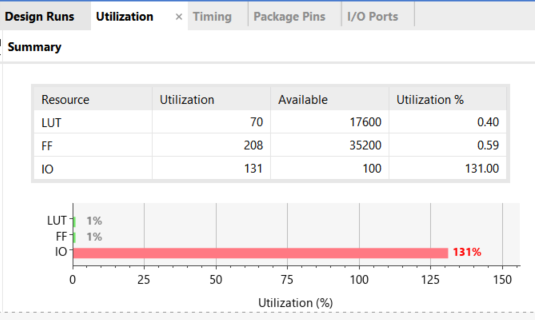
\includegraphics[scale=.75,clip]{img/vivado_lut_resources.png}
    \end{center}
    \vspace*{-0.5cm}
    \caption{Summary of the resource utilization report of the LUT-based architecture}
    \label{fig:vivado_bit_resources}
\end{figure}
\hfill \break
The report obviously present the same issue as before, as far as it concerns the IO utilization.\\
The LUT and FF utilization, surprisingly, are lower. This is thought to be a consequence of the optimizations performed by Vivado during the synthesis process.

\subsection{Power consumption report}

The following figure shows a summary of the power consumption utilization report for the LUT-based architecture.

\begin{figure}[H]
    \begin{center}
        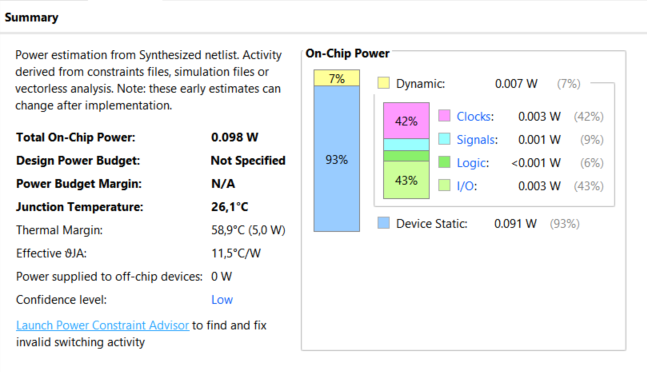
\includegraphics[scale=.85,clip]{img/vivado_lut_power.png}
    \end{center}
    \vspace*{-0.5cm}
    \caption{Summary of the power consumption report of the LUT-based architecture}
    \label{fig:vivado_bit_power}
\end{figure}

The total power absorbed by the chip is again in the order of 0.1 W, although slightly lower than the previous implementation. In this architecture too, most of it is static power consumption.\\
Just as before, this values should be taken with a grain of salt for the same reasons set forth.